\documentclass[10pt,a4papper]{article}
\usepackage{graphicx}
\usepackage{physics}
\usepackage{amsmath}
\usepackage{amssymb}
\usepackage{cancel}
\usepackage{multicol}
\usepackage{blindtext}
\usepackage{tikz}

\usepackage{mathtools}  % <----- for '\mathrlap' command (necessary)

\newcommand{\mybar}[3]{%
    \mathrlap{\hspace{#2}\overline{\scalebox{#1}[1]{\phantom{\ensuremath{#3}}}}}\ensuremath{#3}
}

\newcommand{\rc}{
  \resizebox{!}{1.25ex}{
    \begin{tikzpicture}[>=round cap]
      \clip (0.09em,-0.05ex) rectangle (0.61em,0.81ex);
      \draw [line width=.11ex, <->, rounded corners=0.13ex] (0.1em,0.1ex) .. controls (0.24em,0.4ex) .. (0.35em,0.8ex) .. controls (0.29em,0.725ex) .. (0.25em,0.6ex) .. controls (0.7em,0.8ex) and (0.08em,-0.4ex) .. (0.55em,0.25ex);
    \end{tikzpicture}
  }
}

\newcommand{\brc}{
\resizebox{!}{1.3ex}{
  
\begin{tikzpicture}[>=round cap]
    \clip (0.085em,-0.1ex) rectangle (0.61em,0.875ex);
    \draw [line width=.2ex, <->, rounded corners=0.13ex] (0.1em,0.1ex) .. controls (0.24em,0.4ex) .. (0.35em,0.8ex) .. controls (0.29em,0.725ex) .. (0.25em,0.6ex) .. controls (0.7em,0.8ex) and (0.08em,-0.4ex) .. (0.55em,0.25ex);
  \end{tikzpicture}
}
}

\newcommand{\hrc}{\hat{\brc}}

\newcommand{\AxisRotator}[1][rotate=0]{%
    \tikz [x=0.25cm,y=0.60cm,line width=.2ex,-stealth,#1] \draw (0,0) arc (-150:150:1 and 1);%
}

\newcommand{\AxisRotatorR}[1][rotate=0]{%
    \tikz [x=0.25cm,y=0.60cm,line width=.2ex,-stealth,#1] \draw (0,0) arc (150:-150:1 and 1);%
}

\usepackage[hidelinks]{hyperref}
\usepackage[left=2.00cm, right=3.00cm, top=2.00cm, bottom=2.00cm]{geometry}
\usetikzlibrary{arrows,scopes}
\usetikzlibrary{angles,quotes}
\usetikzlibrary{snakes,shapes}
\usetikzlibrary{decorations.pathreplacing}
\usetikzlibrary{calc}
\tikzset{>=latex}
\setlength{\parindent}{0cm}
\author{Angel Fdo. García Núñez}
\date{Enero 18, 2023}
\title{Estadisitica}

\begin{document}

\Huge
\textbf{Introduction to}\\
\textbf{Electrodynamics}\\

\large
\textbf{Fourth Edition}\\\\\\\\\\\\\\\\

\textbf{David J. Griffiths}\\\\\\\\\\\\\\\\\\\\

\Large
\textbf{Solucionario}\\\\
\large
\textbf{Angel Fernando García Núñez}

\Large
\newpage
\textbf{Problem 1.1} Using the definitions in Eqs. 1.1 and 1.4, and appropriate\\
diagrams, show that the dot product and cross product are distributive,\\

a) when the three vectors are coplanar;\\

b) in the general case.


\newpage
\[\text{Vectores coplanares}\]

\begin{center}
  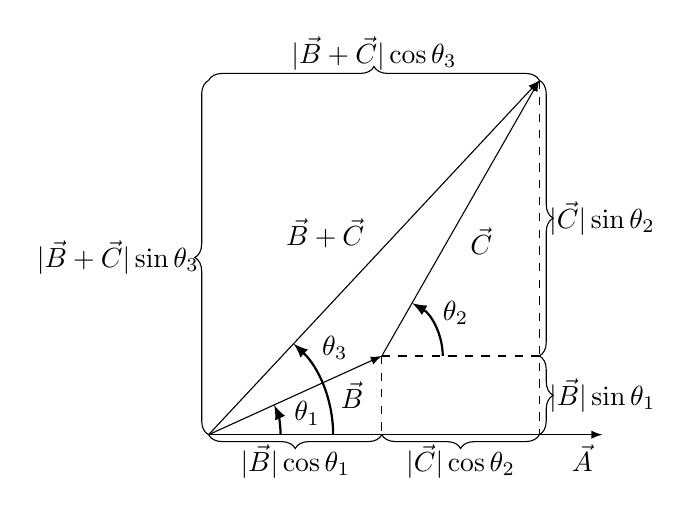
\begin{tikzpicture}
    \coordinate (O) at (0,0);
    \coordinate (A) at (5,0);
    \coordinate (B) at (2.2,1);
    \coordinate (C) at (2,3.5);
    \coordinate (B+C) at ($(B)+(C)$);
    \coordinate (BX) at (2.2,0);
    \coordinate (CX) at (4.2,0);
    \coordinate (BL) at (4.2,1);

    \draw[->](O)--(A) node[below left]{$\vec A$};
    \draw[->](O)--(B) node[midway,right=13]{$\vec B$};
    \draw[->](B)--(B+C) node[midway,below right]{$\vec C$};
    \draw[->](O)--(B+C) node[midway,above left]{$\vec B+\vec C$};
    \draw[dashed](B)--(BL);
    \draw[dashed](B)--(BX);
    \draw[dashed](B+C)--(CX);

    \draw pic[->,thick,"$\theta_1$",draw=black,angle radius=26,angle eccentricity=1.4]{angle=A--O--B};
    \draw pic[->,thick,"$\theta_2$",draw=black,angle radius=22,angle eccentricity=1.4]{angle=BL--B--B+C};
    \draw pic[->,thick,"$\theta_3$",draw=black,angle radius=45,angle eccentricity=1.3,pic text options={shift={(-8pt,8pt)}}]{angle=A--O--B+C};

    %\draw[black,thick,snake=brace] (BX)--(O) node[midway,below]{$|\vec B|\cos\theta_1$};
    %\draw[black,thick,snake=brace] (CX)--(BX) node[midway,below]{$|\vec C|\cos\theta_2$};
    %\draw[black,thick,snake=brace] (BL)--(CX) node[midway,right]{$|\vec B|\sin\theta_1$};
    %\draw[black,thick,snake=brace] (B+C)--(BL) node[midway,right]{$|\vec C|\sin\theta_2$};

    \draw[decorate,decoration={brace,amplitude=5pt}] (BX)--(O) node[midway,below]{$|\vec B|\cos\theta_1$};
    \draw[decorate,decoration={brace,amplitude=5pt}] (CX)--(BX) node[midway,below]{$|\vec C|\cos\theta_2$};
    \draw[decorate,decoration={brace,amplitude=5pt}] (BL)--(CX) node[midway,right]{$|\vec B|\sin\theta_1$};
    \draw[decorate,decoration={brace,amplitude=5pt}] (B+C)--(BL) node[midway,right]{$|\vec C|\sin\theta_2$};
    \draw[decorate,decoration={brace,amplitude=5pt}] (0,4.5)--(B+C) node[midway,above]{$|\vec B+\vec C|\cos\theta_3$};
    \draw[decorate,decoration={brace,amplitude=5pt}] (0,0)--(0,4.5) node[midway,left]{$|\vec B+\vec C|\sin\theta_3$};
  \end{tikzpicture}
\end{center}

Como podemos ver en el diagrama, cuando los vectores $\vec A$, $\vec B$ y $\vec C$ son coplanares
se mantienen las siguientes relaciones:

\[|\vec B|\cos\theta_1+|\vec C|\cos\theta_2=|\vec B+\vec C|\cos\theta_3\]
\[|\vec B|\sin\theta_1+|\vec C|\sin\theta_2=|\vec B+\vec C|\sin\theta_3\]\\

\[\text{Ecuación 1.1}\]

\[\vb{A\cdot B}\equiv AB\cos\theta\]

\[\text{Ecuación 1.4}\]

\[\vb{A\times B}\equiv AB\sin\theta\vb{\hat n}\]

\newpage
\[\text{Propiedad distributiva en el producto escalar}\]

\[\vec A\cdot(\vec B+\vec C)=\vec A\cdot\vec B+\vec A\cdot\vec C\quad?\]\\

\[\vec A\cdot(\vec B+\vec C)=\vec A\cdot\vec B+\vec A\cdot\vec C\quad\to\quad
|\vec A||\vec B+\vec C|\cos\theta_3=|\vec A||\vec B|\cos\theta_1+|\vec A||\vec C|\cos\theta_2\]

\[A=|\vec A|\]

\[A|\vec B+\vec C|\cos\theta_3=A|\vec B|\cos\theta_1+A|\vec C|\cos\theta_2=A\left(|\vec B|\cos\theta_1+|\vec C|\cos\theta_2\right)\]

\[A|\vec B+\vec C|\cos\theta_3=A|\vec B+\vec C|\cos\theta_3\]\\

\[\boxed{\text{1.1 a)}\quad\vec A\cdot(\vec B+\vec C)=\vec A\cdot\vec B+\vec A\cdot\vec C\quad\blacksquare}\]

\newpage
\[\text{Propiedad distributiva en el producto vectorial}\]

\[\vec A\times(\vec B+\vec C)=\vec A\times\vec B+\vec A\times\vec C\quad?\]\\

\[\vec A\times(\vec B+\vec C)=\vec A\times\vec B+\vec A\times\vec C\quad\to\quad
|\vec A||\vec B+\vec C|\cos\theta_3\hat n=|\vec A||\vec B|\cos\theta_1\hat n+|\vec A||\vec C|\sin\theta_2\hat n\]

\[A=|\vec A|\]

\[A|\vec B+\vec C|\sin\theta_3\hat n=A|\vec B|\sin\theta_1\hat n+A|\vec C|\sin\theta_2\hat n=A\left(|\vec B|\sin\theta_1+|\vec C|\sin\theta_2\right)\hat n\]

\[A|\vec B+\vec C|\sin\theta_3\hat n=A|\vec B+\vec C|\sin\theta_3\hat n\]\\

\[\boxed{\text{1.1 a)}\quad\vec A\times(\vec B+\vec C)=\vec A\times\vec B+\vec A\times\vec C\quad\blacksquare}\]

\newpage
\[\text{Caso general}\]

\[\vec A=a_x\hat\imath+a_y\hat\jmath+a_z\hat k\quad,\quad
\vec B=b_x\hat\imath+b_y\hat\jmath+b_z\hat k\quad,\quad
\vec C=c_x\hat\imath+c_y\hat\jmath+c_z\hat k\]

\[\vec B+\vec C=(b_x+c_x)\hat\imath+(b_y+c_y)\hat\jmath+(b_z+c_z)\hat k\]\\

\[\text{Propiedad distributiva en el producto escalar}\]

\[\boxed{\vec A\cdot(\vec B+\vec C)=a_x(b_x+c_x)+a_y(b_y+c_y)+a_z(b_z+c_z)}\]

\[\vec A\cdot\vec B=a_xb_x+a_yb_y+a_zb_z\quad,\quad
\[\vec A\cdot\vec C=a_xc_x+a_yc_y+a_zc_z\]

\[\boxed{\vec A\cdot\vec B+\vec A\cdot\vec C=a_x(b_x+c_x)+a_y(b_y+c_y)+a_z(b_z+c_z)}\]\\

\[\boxed{\text{1.1 b)}\quad\vec A\cdot(\vec B+\vec C)=\vec A\cdot\vec B+\vec A\cdot\vec C\quad\blacksquare}\]

\newpage
\[\text{Propiedad distributiva en el producto vectorial}\]

\[\vec A\times(\vec B+\vec C)=
\begin{vmatrix}
  \hat\imath & \hat\jmath & \hat k\\
  a_x & a_y & a_z\\
  (b_x+c_x) & (b_y+c_y) & (b_z+c_z)
\end{vmatrix}\]

\begin{center}
  \fbox{\begin{minipage}{17cm}
      \[\vec A\times(\vec B+\vec C)=\]
      \[[a_y(b_z+c_z)-a_z(b_y+c_y)]\hat\imath+[a_z(b_x+c_x)-a_x(b_z+c_z)]\hat\jmath+[a_x(b_y+c_y)-a_y(b_x+c_x)]\hat k\]
      \end{minipage}}
\end{center}.\\

\[\vec A\times\vec B=
\begin{vmatrix}
  \hat\imath & \hat\jmath & \hat k\\
  a_x & a_y & a_z\\
  b_x & b_y & b_z
\end{vmatrix}=
\hat\imath(a_yb_z-a_zb_y)-\hat\jmath(a_xb_z-a_zb_x)+\hat k(a_xb_y-a_yb_x)\]

\[\boxed{\vec A\times\vec B=(a_yb_z-a_zb_y)\hat\imath+(a_zb_x-a_xb_z)\hat\jmath+(a_xb_y-a_yb_x)\hat k}\]\\

\[\vec A\times\vec C=
\begin{vmatrix}
  \hat\imath & \hat\jmath & \hat k\\
  a_x & a_y & a_z\\
  c_x & c_y & c_z
\end{vmatrix}=
\hat\imath(a_yc_z-a_zc_y)-\hat\jmath(a_xc_z-a_zc_x)+\hat k(a_xc_y-a_yc_x)\]

\[\boxed{\vec A\times\vec C=(a_yc_z-a_zc_y)\hat\imath+(a_zc_x-a_xc_z)\hat\jmath+(a_xc_y-a_yc_x)\hat k}\]\\


\begin{center}
  \fbox{\begin{minipage}{17cm}
      \[\vec A\times\vec B+\vec A\times\vec C=\]
      \[[a_y(b_z+c_z)-a_z(b_y+c_y)]\hat\imath+[a_z(b_x+c_x)-a_x(b_z+c_z)]\hat\jmath+[a_x(b_y+c_y)-a_y(b_x+c_x)]\hat k\]
      \end{minipage}}
\end{center}.\\

\[\boxed{\text{1.1 b)}\quad\vec A\times(\vec B+\vec C)=\vec A\times\vec B+\vec A\times\vec C\quad\blacksquare}\]

\newpage
\textbf{Problem 1.2} Is the cross product associative?

\[\vb{(A\times B)\times C\overset{?}=A\times(B\times C)}.\] 

If so, \textit{prove} it; if not, provide a counterexample (the simpler the better).

\newpage
\[(\vec A\times\vec B)\times\vec C=\vec A\times(\vec B\times\vec C)\quad?\]

\[\vec A=a_x\hat\imath+a_y\hat\jmath+a_z\hat k\quad,\quad
\vec B=b_x\hat\imath+b_y\hat\jmath+b_z\hat k\quad,\quad
\vec C=c_x\hat\imath+c_y\hat\jmath+c_z\hat k\]

\[\vec A\times\vec B=
\begin{vmatrix}
  \hat\imath & \hat\jmath & \hat k\\
  a_x & a_y & a_z\\
  b_x & b_y & b_z
\end{vmatrix}=
\hat\imath(a_yb_z-a_zb_y)-\hat\jmath(a_xb_z-a_zb_x)+\hat k(a_xb_y-a_yb_x)\]\\

\[\boxed{\vec A\times\vec B=(a_yb_z-a_zb_y)\hat\imath+(a_zb_x-a_xb_z)\hat\jmath+(a_xb_y-a_yb_x)\hat k}\]\\

\[(\vec A\times\vec B)\times\vec C=
\begin{vmatrix}
  \hat\imath & \hat\jmath & \hat k\\
  (a_yb_z-a_zb_y) & (a_zb_x-a_xb_z) & (a_xb_y-a_yb_x)\\
  c_x & c_y & c_z
\end{vmatrix}\]\\

\[(\vec A\times\vec B)\times\vec C=\]
\[\hat\imath[(a_zb_x-a_xb_z)c_z-(a_xb_y-a_yb_x)c_y]\]
\[-\hat\jmath[(a_yb_z-a_zb_y)c_z-(a_xb_y-a_yb_x)c_x]\]
\[+\hat k[(a_yb_z-a_zb_y)c_y-(a_zb_x-a_xb_z)c_x]\]\\

\begin{center}
  \fbox{\begin{minipage}{8cm}
      \[(\vec A\times\vec B)\times\vec C=\]
      \[[(a_zb_x-a_xb_z)c_z-(a_xb_y-a_yb_x)c_y]\hat\imath\]
      \[+[(a_xb_y-a_yb_x)c_x-(a_yb_z-a_zb_y)c_z]\hat\jmath\]
      \[+[(a_yb_z-a_zb_y)c_y-(a_zb_x-a_xb_z)c_x]\hat k\]
  \end{minipage}}
\end{center}

\newpage
\[\vec B\times\vec C=
\begin{vmatrix}
  \hat\imath & \hat\jmath & \hat k\\
  b_x & b_y & b_z\\
  c_x & c_y & c_z
\end{vmatrix}=
\hat\imath(b_yc_z-b_zc_y)-\hat\jmath(b_xc_z-b_zc_x)+\hat k(b_xc_y-b_yc_x)\]\\

\[\boxed{\vec B\times\vec C=(b_yc_z-b_zc_y)\hat\imath+(b_zc_x-b_xc_z)\hat\jmath+(b_xc_y-b_yc_x)\hat k}\]\\

\[\vec A\times(\vec B\times\vec C)=
\begin{vmatrix}
  \hat\imath & \hat\jmath & \hat k\\
  a_x & a_y & a_z\\
  (b_yc_z-b_zc_y) & (b_zc_x-b_xc_z) & (b_xc_y-b_yc_x)
\end{vmatrix}\]\\

\[\vec A\times(\vec B\times\vec C)=\]
\[\hat\imath[(b_xc_y-b_yc_x)a_y-(b_zc_x-b_xc_z)a_z]\]
\[-\hat\jmath[(b_xc_y-b_yc_x)a_x-(b_yc_z-b_zc_y)a_z]\]
\[+\hat k[(b_zc_x-b_xc_z)a_x-(b_yc_z-b_zc_y)a_y]\]\\

\begin{center}
  \fbox{\begin{minipage}{8cm}
      \[\vec A\times(\vec B\times\vec C)=\]
      \[[(b_xc_y-b_yc_x)a_y-(b_zc_x-b_xc_z)a_z]\hat\imath\]
      \[+[(b_yc_z-b_zc_y)a_z-(b_xc_y-b_yc_x)a_x]\hat\jmath\]
      \[+[(b_zc_x-b_xc_z)a_x-(b_yc_z-b_zc_y)a_y]\hat k\]
      \end{minipage}}
\end{center}

\newpage
\[(a_zb_x-a_xb_z)c_z-(a_xb_y-a_yb_x)c_y\not=(b_xc_y-b_yc_x)a_y-(b_zc_x-b_xc_z)a_z\]
\[(a_xb_y-a_yb_x)c_x-(a_yb_z-a_zb_y)c_z\not=(b_yc_z-b_zc_y)a_z-(b_xc_y-b_yc_x)a_x\]
\[(a_yb_z-a_zb_y)c_y-(a_zb_x-a_xb_z)c_x\not=(b_zc_x-b_xc_z)a_x-(b_yc_z-b_zc_y)a_y\]

\[\therefore\quad(\vec A\times\vec B)\times\vec C\not=\vec A\times(\vec B\times\vec C)\]\\

\begin{center}
  \fbox{\begin{minipage}{9cm}
      1.2
      \[(\vec A\times\vec B)\times\vec C\not=\vec A\times(\vec B\times\vec C)\quad\blacksquare\]
      \[\text{El producto vectorial es no asociativo.}\]
      \end{minipage}}
\end{center}

\newpage
\textbf{Problem 1.3} Find the angle between the body diagonals of a cube.

\newpage
Supondremos un cubo con arista de longitud $a$, con vertices en $(0,0,0)$,
$(a,0,0)$, $(0,a,0)$, $(0,0,a)$, $(a,a,0)$, $(0,a,a)$, $(a,0,a)$, y $(a,a,a)$, siendo las
diagonales aquellos vectores $\vec A$ de $(0,0,0)$ a $(a,a,a)$, y $\vec B$ de $(0,0,a)$ a $(a,a,0)$.\\

\[\text{Vectores posicionados en el origen}\]

\[\vec A=a\hat\imath+a\hat\jmath+a\hat k\quad,\quad\vec B=a\hat\imath+a\hat\jmath-a\hat k\]

\[\text{Magnitudes}\]

\[A=|\vec A|=\sqrt{a^2+a^2+a^2}=\sqrt{3}a\]

\[B=|\vec B|=\sqrt{a^2+a^2+(-a)^2}=\sqrt{3}a\]

\[\text{Producto escalar}\]

\[\vec A\cdot\vec B=a^2+a^2-a^2=a^2\]

\[\vec A\cdot\vec B=AB\cos\theta\quad\to\quad\theta=\acos\left(\frac{\vec A\cdot\vec B}{AB}\right)\]\\

\[\theta=\acos\left(\frac{a^2}{(\sqrt{3}a)(\sqrt{3}a)}\right)=\acos\left(\frac{1}{2}\right)\]\\

\[\boxed{\text{1.3}\quad\theta\approx 1.231\text{rad}}\]

\newpage
\textbf{Problem 1.4} Use the cross product to find the components of the unit vector
$\vb{\hat n}$ perpendicular to the shaded plane in Fig 1.11.

\newpage
En el plano de la figura 1.11 están ubicados los vertices $(1,0,0)$, $(0,2,0)$, y
$(0,0,3)$, por lo que tomaremos los vectores $\vec A$ de $(1,0,0)$ a $(0,2,0)$, y $\vec B$ de
$(1,0,0)$ a $(0,0,3)$.

\[\text{Vectores posicionados en el origen}\]

\[\vec A=-1\hat\imath+2\hat\jmath+0\hat k\quad,\quad\vec B=-1\hat\imath+0\hat\jmath+3\hat k\]

\[\text{Producto vectorial - vector normal}\]

\[\vec n=\vec A\times\vec B\]

\[\vec n=
\begin{vmatrix}
  \hat\imath & \hat\jmath & \hat k\\
  -1 & 2 & 0\\
  -1 & 0 & 3
\end{vmatrix}=[2(3)-0]\hat\imath-[-1(3)-0]\hat\jmath+[0-2(-1)]\hat k\]

\[\vec n=6\hat\imath+3\hat\jmath+2\hat k\]

\[n=|\vec n|=\sqrt{6^2+3^2+2^2}=7\]\\

\[\text{Vector normal unitario}\]

\[\hat n=\frac{\vec n}{n}=\frac{1}{7}(6\hat\imath+3\hat\jmath+2\hat k)\]\\

\[\boxed{\text{1.4}\quad\hat n=\frac{6}{7}\hat\imath+\frac{3}{7}\hat\jmath+\frac{2}{7}\hat k}\]

\newpage
\textbf{Problem 1.5} Prove the \textbf{BAC-CAB} rule by writing out both sides in\\
component form.

\newpage
\[\vec A\times(\vec B\times\vec C)=\vec B(\vec A\cdot\vec C)-\vec C(\vec A\cdot\vec B)\quad?\]\\

\[\vec A\times(\vec B\times\vec C)=\]
\[[(b_xc_y-b_yc_x)a_y-(b_zc_x-b_xc_z)a_z]\hat\imath\]
\[+[(b_yc_z-b_zc_y)a_z-(b_xc_y-b_yc_x)a_x]\hat\jmath\]
\[+[(b_zc_x-b_xc_z)a_x-(b_yc_z-b_zc_y)a_y]\hat k\]\\

\[\vec B(\vec A\cdot\vec C)=(a_xc_x+a_yc_y+a_zc_z)(b_x\hat\imath+b_y\hat\jmath+b_z\hat k)\]

\[\vec C(\vec A\cdot\vec B)=(a_xb_x+a_yb_y+a_zb_z)(c_x\hat\imath+c_y\hat\jmath+c_z\hat k)\]

\[\vec B(\vec A\cdot\vec C)-\vec C(\vec A\cdot\vec B)=\]
\[[(a_yc_y+a_zc_z)b_x-(a_yb_y+a_zb_z)c_x]\hat\imath\]
\[+[(a_xc_x+a_zc_z)b_y-(a_xb_x+a_zb_z)c_y]\hat\jmath\]
\[+[(a_xc_x+a_yc_y)b_z-(a_xb_x+a_yb_y)c_z]\hat k=\]

\[(a_yc_yb_x+a_zc_zb_x-a_yb_yc_x-a_zb_zc_x)\hat\imath\]
\[+(a_xc_xb_y+a_zc_zb_y-a_xb_xc_y-a_zb_zc_y)\hat\jmath\]
\[+(a_xc_xb_z+a_yc_yb_z-a_xb_xc_z-a_yb_yc_z)\hat k\]

\[\vec B(\vec A\cdot\vec C)-\vec C(\vec A\cdot\vec B)=\]
\[[(b_xc_y-b_yc_x)a_y-(b_zc_x-b_xc_z)a_z]\hat\imath\]
\[+[(b_yc_z-b_zc_y)a_z-(b_xc_y-b_yc_x)a_x]\hat\jmath\]
\[+[(b_zc_x-b_xc_z)a_x-(b_yc_z-b_zc_y)a_y]\hat k\]\\

\[\boxed{\text{1.5}\quad\vec A\times(\vec B\times\vec C)=\vec B(\vec A\cdot\vec C)-\vec C(\vec A\cdot\vec B)\quad\blacksquare}\]

\newpage
\textbf{Problem 1.6} Prove that

\[\vb{[A\times(B\times C)]+[B\times(C\times A)]+[C\times(A\times B)]=0}\]

Under what conditions does $\vb{A\times(B\times C)=(A\times B)\times C}$?

\newpage
\[[\vec A\times(\vec B\times\vec C)]+[\vec B\times(\vec C\times\vec A)]+[\vec C\times(\vec A\times\vec B)]=0\quad?\]\\

\[\vec A\times(\vec B\times\vec C)=\vec B(\vec A\cdot\vec C)-\vec C(\vec A\cdot\vec B)\]

\[\vec B\times(\vec C\times\vec A)=\vec C(\vec B\cdot\vec A)-\vec A(\vec B\cdot\vec C)\]

\[\vec C\times(\vec A\times\vec B)=\vec A(\vec C\cdot\vec B)-\vec B(\vec C\cdot\vec A)\]\\

\[\vec A\times(\vec B\times\vec C)+\vec B\times(\vec C\times\vec A)+\vec C\times(\vec A\times\vec B)=\]
\[\vec B(\vec A\cdot\vec C)-\vec C(\vec A\cdot\vec B)+\vec C(\vec B\cdot\vec A)-\vec A(\vec B\cdot\vec C)+\vec A(\vec C\cdot\vec B)-\vec B(\vec C\cdot\vec A)=\]
\[\vec B(\vec A\cdot\vec C)-\vec C(\vec A\cdot\vec B)+\vec C(\vec A\cdot\vec B)-\vec A(\vec B\cdot\vec C)+\vec A(\vec B\cdot\vec C)-\vec B(\vec A\cdot\vec C)\]\\

\[\boxed{\text{1.6}\quad[\vec A\times(\vec B\times\vec C)]+[\vec B\times(\vec C\times\vec A)]+[\vec C\times(\vec A\times\vec B)]=0\quad\blacksquare}\]

\newpage
\[\vec A\times(\vec B\times\vec C)=(\vec A\times\vec B)\times\vec C\quad?\]\\

\[\vec A\times(\vec B\times\vec C)=\vec B(\vec A\cdot\vec C)-\vec C(\vec A\cdot\vec B)\]

\[(\vec A\times\vec B)\times\vec C=-\vec C\times(\vec A\times\vec B)=\vec B(\vec C\cdot\vec A)-\vec A(\vec C\cdot\vec B)\]\\

\[\boxed{\vec A\cdot\vec B\not=\vec C\cdot\vec B\not=0}\]

\[\vec C(\vec A\cdot\vec B)=\vec A(\vec C\cdot\vec B)\quad\to\quad\vec A\parallel\vec C\quad\to\quad\vec A\cdot\vec C=|\vec A||\vec C|\]\\

\begin{center}
  \fbox{\begin{minipage}{16cm}
      1.6
      \[(\vec A\times\vec B)\times\vec C=\vec A\times(\vec B\times\vec C)\quad:\quad
      \vec A\cdot\vec B=\vec C\cdot\vec B=0\quad\cup\quad\vec A\cdot\vec C=\pm|\vec A||\vec C|\]
      La propiedad se cumple si $\vec B$ es perpendicular con $\vec A$ y $\vec C$, o que $\vec A$ y $\vec C$ sean paralelos.
      \end{minipage}}
\end{center}

\newpage
\textbf{Problem 1.7} Find the separation vector $\brc$ from the source point $(2,8,7)$ to
the field point $(4,6,8)$. Determine its magnitude $(\rc)$, and construct the unit
vector $\hrc$.

\newpage
\[\text{Vector de separación}\]

\[\vec\rc=\vec r-\vec{r}'\]\\

\[\vec r=(4,6,8)\quad,\quad\vec r'=(2,8,7)\quad\to\quad\vec\rc=(2,-2,1)\]

\[\rc=|\vec\rc|\quad\to\quad\rc=\sqrt{2^2+(-2)^2+1^2}=3\]

\[\hat\rc=\frac{\vec\rc}{\rc}=\frac{1}{3}(2,-2,1)\]\\

\[\boxed{\text{1.7}\quad\hat\rc=\left(\frac{2}{3},-\frac{2}{3},\frac{1}{3}\right)}\]

\newpage
\textbf{Problem 1.8}\\

(a) Prove that the two-dimensional rotation matrix (Eq. 1.29) preserves dot
products. (That is, show that $\mybar{0.6}{3pt}{A_y}\mybar{0.6}{3pt}{B_y}+\mybar{0.6}{3pt}{A_z}\mybar{0.6}{3pt}{B_z}=A_yB_y+A_zB_z$.)\\

(b) What constraints must the element $(R_{ij})$ of the three-dimensional rotation
matrix (Eq. 1.30) satisfy, in order to preserve the length of $\vb{A}$ (for all vectors
$\vb{A}$)?

\newpage
\[\text{Ecuación 1.29}\]

\[\begin{pmatrix}
\mybar{0.6}{3pt}{A_x}\\
\mybar{0.6}{3pt}{A_z}
\end{pmatrix}=
\begin{pmatrix}
  \cos\phi & \sin\phi\\
  -\sin\phi & \cos\phi
\end{pmatrix}
\begin{pmatrix}
  A_x\\
  A_z
\end{pmatrix}\]\\

\[P_\phi=
\begin{pmatrix}
  \cos\phi & \sin\phi\\
  -\sin\phi & \cos\phi
\end{pmatrix}\]\\

\[\vec A\cdot\vec B=\left(P_\phi\vec A\right)\cdot\left(P_\phi\vec B\right)\quad?\]\\

\[\bar A_x=A_x\cos\phi+A_z\sin\phi\quad,\quad\bar A_z=-A_x\sin\phi+A_z\cos\phi\]
\[\bar B_x=B_x\cos\phi+B_z\sin\phi\quad,\quad\bar B_z=-B_x\sin\phi+B_z\cos\phi\]\\

\[\left(P_\phi\vec A\right)\cdot\left(P_\phi\vec B\right)=\bar A_x\bar B_x+\bar A_z\bar B_z=\]
\[(A_x\cos\phi+A_z\sin\phi)(B_x\cos\phi+B_z\sin\phi)+(-A_x\sin\phi+A_z\cos\phi)(-B_x\sin\phi+B_z\cos\phi)\]

\[\left(P_\phi\vec A\right)\cdot\left(P_\phi\vec B\right)=\]
\[A_xB_x\cos^2\phi+A_xB_z\cos\phi\sin\phi+A_zB_x\cos\phi\sin\phi+A_zB_z\sin^2\phi\]
\[A_xB_x\sin^2\phi-A_xB_z\cos\phi\sin\phi-A_zB_x\cos\phi\sin\phi+A_zB_z\cos^2\phi\]

\[\left(P_\phi\vec A\right)\cdot\left(P_\phi\vec B\right)=(A_xB_x+A_zB_z)(\cos^2\phi+\sin^2\phi)=A_xB_x+A_zB_z\]\\

\[\boxed{\text{1.8 (a)}\quad\vec A\cdot\vec B=\left(P_\phi\vec A\right)\cdot\left(P_\phi\vec B\right)\quad\blacksquare}\]

\newpage
\[\text{Ecuación 1.30}\]

\[\begin{pmatrix}
\mybar{0.6}{3pt}{A_x}\\
\mybar{0.6}{3pt}{A_y}\\
\mybar{0.6}{3pt}{A_z}
\end{pmatrix}=
\begin{pmatrix}
  R_{xx} & R_{xy} & R_{xz}\\
  R_{yx} & R_{yy} & R_{yz}\\
  R_{zx} & R_{zy} & R_{zz}
\end{pmatrix}
\begin{pmatrix}
  A_x\\
  A_y\\
  A_z
\end{pmatrix}\]\\

\[\bar A_i=\sum_jR_{ij}A_j\]\\

\[|\vec A|^2=\vec A\cdot\vec A=A_x^2+A_y^2+A_z^2=\bar A_x^2+\bar A_y^2+\bar A_z^2\]

\[\sum_iA_i^2=\left(\sum_jR_{xj}A_j\right)^2+\left(\sum_jR_{yj}A_j\right)^2+\left(\sum_jR_{zj}A_j\right)^2\]\\

\[\sum_iA_i^2=\sum_i\left(\sum_jR_{ij}A_j\right)^2=\sum_i\left(\sum_jR_{ij}A_j\right)\left(\sum_kR_{ik}A_k\right)\]\\

\[\sum_iA_i^2=\sum_i\sum_{j,k}R_{ij}R_{ik}A_jA_k=\sum_{j,k}A_jA_k\sum_iR_{ij}R_{ik}\]

\[\boxed{\sum_iR_{ij}R_{ik}=\delta_{jk}}\]

\[\sum_iA_i^2=\sum_{j,k}A_jA_k\delta_{jk}=\sum_iA_iA_i=\sum_iA_i^2\]\\

\[\boxed{\text{1.8 (b)}\quad
  \text{Restricción:}\quad
  \sum_iR_{ij}R_{ik}=
  \delta_{jk}=
  \left\{\begin{array}{lll}
  0 & : & j\not=k\\
  1 & : & j=k
  \end{array}\right.}\]

\newpage
\textbf{Problem 1.9} Find the transformation matrix $R$ that describes a rotation
by $120^\circ$ about an axis from the origin through the point $(1,1,1)$. The rotation
is clockwise as you look down the axis toward the origin.

\newpage
\[\text{Transformación de la matriz }R\]\\

\begin{center}
  \begin{tikzpicture}
    \coordinate (O) at (0,0);
    \coordinate (X) at (2,0);
    \coordinate (Y) at (0,2);
    \coordinate (Z) at ({-1.5*cos(45)},{-1.5*sin(45)});
    \coordinate (P) at (1,1.5);

    \coordinate (O') at (7,0);
    \coordinate (X') at (9,0);
    \coordinate (Y') at (7,2);
    \coordinate (Z') at ({-1.5*cos(45)+7},{-1.5*sin(45)});

    \draw[->](O)--(X) node[below]{$x$};
    \draw[->](O)--(Y) node[above left]{$y$};
    \draw[->](O)--(Z) node[below left]{$z$};
    \draw[->](O)--(P) node[midway]{\AxisRotatorR[x=0.2cm,y=0.25cm,rotate=-45]} node[below right]{$120^\circ$} node[above right]{$(1,1,1)$};

    \draw[->](3,1)--(5,1);

    \draw[->](O')--(X') node[below]{$y'$};
    \draw[->](O')--(Y') node[above left]{$z'$};
    \draw[->](O')--(Z') node[below left]{$x'$};
  \end{tikzpicture}
\end{center}

\[\boxed{\therefore\quad\bar A_x=A_z\quad,\quad\bar A_z=A_y\quad,\quad\bar A_y=A_x}\]\\

\[\bar A_i=\sum_jR_{ij}A_j\]\\

\[\bar A_x=R_{xx}A_x+R_{xy}A_y+R_{xz}A_z=A_z\quad\to\quad
\quad R_{xx}=R_{xy}=0\quad,\quad R_{xz}=1\]

\[\bar A_y=R_{yx}A_x+R_{yy}A_y+R_{yz}A_z=A_x\quad\to\quad
\quad R_{yy}=R_{yz}=0\quad,\quad R_{yx}=1\]

\[\bar A_z=R_{zx}A_x+R_{zy}A_y+R_{zz}A_z=A_y\quad\to\quad
\quad R_{zx}=R_{zz}=0\quad,\quad R_{zy}=1\]\\

\[\boxed{\text{1.9}\quad
  R=
  \begin{pmatrix}
    0 & 0 & 1\\
    1 & 0 & 0\\
    0 & 1 & 0
  \end{pmatrix}}\]

\newpage
\textbf{Problem 1.10}\\

(a) How do the components of a vector$^5$ transform under a \textbf{translation} of
coordinates $(\mybar{1.0}{0pt}{x}=x,\mybar{1.0}{0pt}{y}=y-a,\mybar{1.0}{0pt}{z}=z$, Fig. 1.16a)?\\

(b) How do the components of a vector transform under an \textbf{inversion} of coordinates
$(\mybar{1.0}{0pt}{x}=-x,\mybar{1.0}{0pt}{y}=-y,\mybar{1.0}{0pt}{z}=-z$, Fig. 1.16b)?\\

(c) How do the components of a cross product (Eq. 1.13) transform under
inversion? [The cross-product of two vectors is properly called a \textbf{pseudovector}
  because of this ``anomalous'' behavoir.] Is the croos product of two pseudovectors
a vector, or a pseudovector? Name two pseudovector quantities in
classical mechanics.\\

(d) How does the scalar triple product of three vectors transform under
inversions? (Such an object is called a \textbf{pseudoscalar.})\\\\\\\\\\\\\\

\begin{center}
  \begin{tikzpicture}
    \coordinate (O) at (0,0);
    \coordinate (Y) at (2,0);
    \coordinate (Z) at (0,2);
    \coordinate (X) at ({-1.5*cos(45)},{-1.5*sin(45)});

    \coordinate (O') at (0.8,0.1);
    \coordinate (Y') at (2.8,0.1);
    \coordinate (Z') at (0.8,2.1);
    \coordinate (X') at ({-1.5*cos(45)+0.8},{-1.5*sin(45)+0.1});

    \coordinate (Op) at (8,0);
    \coordinate (Yp) at (10,0);
    \coordinate (Zp) at (8,1.5);
    \coordinate (Xp) at ({-1.5*cos(45)+8},{-1.5*sin(45)});

    \coordinate (Op') at (7.9,0);
    \coordinate (Yp') at (5.9,0);
    \coordinate (Zp') at (7.9,-1.5);
    \coordinate (Xp') at ({1.5*cos(45)+7.9},{1.5*sin(45)});
    
    \draw[->](O)--(Y) node[below]{$y$};
    \draw[->](O)--(Z) node[left]{$z$};
    \draw[->](O)--(X) node[left]{$x$};

    \draw[->](O')--(Y') node[above]{$\mybar{1.0}{0pt}{y}$};
    \draw[->](O')--(Z') node[left]{$\mybar{1.0}{0pt}{z}$};
    \draw[->](O')--(X') node[left]{$\mybar{1.0}{0pt}{x}$};

    \node[draw=none] at (2.5,-1.5){(a)};

    \draw[decorate,decoration={brace,amplitude=5pt}] (0,0)--(0.8,0) node[midway,above=3]{$a$};

    \draw[->](Op)--(Yp) node[above]{$y$};
    \draw[->](Op)--(Zp) node[left]{$z$};
    \draw[->](Op)--(Xp) node[left]{$x$};

    \draw[->](Op')--(Yp') node[above]{$\mybar{1.0}{0pt}{y}$};
    \draw[->](Op')--(Zp') node[left]{$\mybar{1.0}{0pt}{z}$};
    \draw[->](Op')--(Xp') node[left]{$\mybar{1.0}{0pt}{x}$};

    \node[draw=none] at (9.5,-1.5){(b)};
    
  \end{tikzpicture}
\end{center}
\[\textbf{FIGURE 1.16}\]

\hline
\hline.\\

$^5$\emph{Beware:} The vector $\vb{r}$ (Eq. 1.19) goes from a specific point in space (the
origin, $\mathcal{O}$) to the point $P=(x,y,z)$. Under translations the \emph{new} origin $(\bar{\mathcal{O}})$
is at a different location, and the arrow from $\bar{\mathcal{O}}$ to $P$ is a completely different
vector. The original vector $\vb{r}$ still goes from $\mathcal{O}$ to $P$, regardless of
the coordinates used to label these points.

\newpage
\begin{center}
  \fbox{\begin{minipage}{17cm}
      1.10 (a)\\
      Si ocurre una traslación del vector $\vec A$ a otro origen, las componentes en la nueva
      base no cambian:
      \[\vec A'\to\vec A\]
      \[\bar A_x=A_x\quad,\quad\bar A_y=A_y\quad,\quad\bar A_z=A_z\]
      \end{minipage}}
\end{center}

\begin{center}
  \fbox{\begin{minipage}{17cm}
      1.10 (b)\\
      En el caso de una inversión, el sentido del vector se invierte al opuesto del
      original, lo que equivale a multiplicarlo por $(-1)$:
      \[\vec A'\to -\vec A\]
      \[\bar A_x=-A_x\quad,\quad\bar A_y=-A_y\quad,\quad\bar A_z=-A_z\]
      \end{minipage}}
\end{center}.\\

\[\text{Ecuación 1.13}\]

\[\vb{A\times B}=(A_x\vb{\hat x}+A_y\vb{\hat y}+A_z\vb{\hat z})\times(B_x\vb{\hat x}+B_y\vb{\hat y}+B_z\vb{\hat z})\]
\[=(A_yB_z-A_zB_y)\vb{\hat x}+(A_zB_x-A_xB_z)\vb{\hat y}+(A_xB_y-A_yB_x)\vb{\hat z}\]

\[\text{Inversión}\]

\[\vec A'\to -\vec A\quad,\quad\vec B'\to -\vec B\]

\[\vec C=\vec A\times\vec B\]

\[\vec C'=\vec A'\times\vec B'=(-\vec A)\times(-\vec B)=\vec A\times\vec B\]

\[\therefore\quad\vec C'\to\vec C\]

\begin{center}
\end{center}

\begin{center}
  \fbox{\begin{minipage}{17cm}
      1.10 (c)\\
      En el caso de una transformación por inversión, tenemos que para el vector
      resultante del producto vectorial de dos vectores ($\vec C=\vec A\times\vec B$) no ocurre inversión,
      sus componentes permanecen iguales, por ello se considera un pseudovector.
      \end{minipage}}
\end{center}

\newpage
\[\text{Tomamos a $\vec A$ y $\vec B$ como pseudovectores}\]

\[\vec A'\to\vec A\quad,\quad\vec B'\to\vec B\]

\[\vec C=\vec A\times\vec B\]

\[\vec C'=\vec A'\times\vec B'=(\vec A)\times(\vec B)=\vec A\times\vec B\]

\[\therefore\quad\vec C'\to\vec C\]

\begin{center}
  \fbox{\begin{minipage}{18cm}
      1.10 (c)\\
      En el caso de una transformación por inversión, tenemos que para el vector
      resultante del producto vectorial de dos pseudovectores ($\vec C=\vec A\times\vec B$) no ocurre
      inversión, sus componentes permanecen iguales, por ello se considera un pseudovector.
      \end{minipage}}
\end{center}.\\

\[\text{Tomamos a $\vec A$ como pseudovector}\]

\[\vec A'\to\vec A\quad,\quad\vec B'\to -\vec B\]

\[\vec C=\vec A\times\vec B\]

\[\vec C'=\vec A'\times\vec B'=(\vec A)\times(-\vec B)=-\vec A\times\vec B\]

\[\therefore\quad\vec C'\to -\vec C\]

\begin{center}
  \fbox{\begin{minipage}{18cm}
      1.10 (c)\\
      En el caso de una transformación por inversión, tenemos que para el vector
      resultante del producto vectorial de un vector y un pseudovector ($\vec C=\vec A\times\vec B$) ocurre inversión,
      por ello se considera un vector ``ordinario''.
      \end{minipage}}
\end{center}

\newpage
\begin{center}
  \fbox{\begin{minipage}{14cm}
      1.10 (c)\\
      \[\text{Ejemplos de pseudovectores en la mecánica clásica:}\]
      
      \[\text{Momento angular:}\quad\vec L=\vec r\times\vec p\]
      \[\text{Momento de torsión:}\quad\vec M=\vec r\times\vec F\]\\
      
      \end{minipage}}
\end{center}.\\

\[\text{Triple producto escalar}\]

\[c=\vec A\cdot(\vec B\times\vec C)\]

\[c'=\vec A'\cdot(\vec B'\times\vec C')=(-\vec A)\cdot[(-\vec B)\times(-\vec C)]=-\vec A\cdot(\vec B\times\vec C)=c\]

\[\therefore\quad c'\to -c\]

\begin{center}
  \fbox{\begin{minipage}{18cm}
      1.10 (d)\\
      En el caso de una transformación por inversión, el pseudoescalar resultante del producto triple
      producto escalar de tres vectores ($c=\vec A\cdot(\vec B\times\vec C)$) invierte su signo.
      \end{minipage}}
\end{center}

\newpage
\textbf{Problem 1.11} Find the gradients of the following functions:\\

(a) $f(x,y,z)=x^2+y^3+z^4$.\\

(b) $f(x,y,z)=x^2y^3z^4$.\\

(c) $f(x,y,z)=e^x\sin(y)\ln(z)$.

\newpage
\[\text{Gradiente de una función}\]

\[\nabla f(x,y,z)=\frac{\partial f}{\partial x}\hat\imath+\frac{\partial f}{\partial y}\hat\jmath+\frac{\partial f}{\partial z}\hat k\]\\

\[f(x,y,z)=x^2+y^3+z^4\quad\to\quad
\frac{\partial f}{\partial x}=2x\quad,\quad
\frac{\partial f}{\partial y}=3y^2\quad,\quad
\frac{\partial f}{\partial z}=4z^3\]\\

\[\boxed{\text{1.11 (a)}\quad\nabla f=2x\hat\imath+3y^2\hat\jmath+4z^3\hat k}\]\\

\[f(x,y,z)=x^2y^3z^4\quad\to\quad
\frac{\partial f}{\partial x}=2xy^3z^4\quad,\quad
\frac{\partial f}{\partial y}=3x^2y^2z^4\quad,\quad
\frac{\partial f}{\partial z}=4x^2y^3z^3\]\\

\[\boxed{\text{1.11 (b)}\quad\nabla f=2xy^3z^4\hat\imath+3x^2y^2z^4\hat\jmath+4x^2y^3z^3\hat k}\]\\

\[f(x,y,z)=e^x\sin y\ln z\]

\[\frac{\partial f}{\partial x}=e^x\sin y\ln z\quad,\quad
\frac{\partial f}{\partial y}=-e^x\cos y\ln z\quad,\quad
\frac{\partial f}{\partial z}=\frac{1}{z}e^x\sin y\]\\

\[\boxed{\text{1.11 (c)}\quad\nabla f=e^x\sin y\ln z\hat\imath-e^x\cos y\ln z\hat\jmath+\frac{1}{z}e^x\sin y\hat k}\]

\newpage
\textbf{Problem 1.12} The height of a certain hill (in feet) is given by

\[h(x,y)=10(2xy-3x^2-4y^2-18x+28y+12),\]

where $y$ is the distance (in miles) north, x the distance east of South Hadley.\\

(a) Where is the top of the hill located?\\

(b) How high is the hill?\\

(c) How steep is the slope (in feet per mile) at a point 1 mile north and one
mile east of South Hadley? In what direction is the slope steepest, at that
point?

\newpage
\[\text{Punto critico}\]

\[\nabla f=\vec 0\quad\to\qua|\nabla f|=0\]\\

\[h(x,y)=10(2xy-3x^2-4y^2-18x+28y+12)\]\\

\[\frac{\partial h}{\partial x}=10(2y-6x-18)\quad,\quad
\frac{\partial h}{\partial y}=10(2x-8y+28)\]\\

\[\therefore\quad\nabla h(x,y)=10(2y-6x-18)\hat\imath+10(2x-8y+28)\hat\jmath\]\\

\[\nabla h=\vec 0=0\hat\imath+0\hat\jmath\]

\[10(2y-6x-18)=0\quad,\quad 10(2x-8y+28)=0\]\\

\[y-3x=9\quad,\quad x-4y=-14\]

\[y=3x+9\quad\to\quad x-4(3x+9)=-14\quad\to\quad -11x=22\quad\to\quad x=-2\]

\[y=3(-2)+9=3\]

\begin{center}
  \fbox{\begin{minipage}{15cm}
      1.12 (a)
      \[x=-2\quad,\quad y=3\]
      La cima se encuentra 3 millas al norte y 2 al oeste de South Hadley.
      \end{minipage}}
\end{center}

\newpage

\[h(-2,3)=10[2(-2)(3)-3(-2)^2-4(3)^2-18(-2)+28(3)+12]=720\]\\

\begin{center}
  \fbox{\begin{minipage}{8cm}
      1.12 (b)
      \[h(-2,3)=720\quad\to\quad h=720\text{ft}\]
      La altura en la cima es de 720 pies.
      \end{minipage}}
\end{center}.\\\\

\[\nabla h(1,1)=
10[2(1)-6(1)-18]\hat\imath+10[2(1)-8(1)+28]\hat\jmath=
10[2-6-18]\hat\imath+10[2-8+28]\hat\jmath\]

\[\boxed{\nabla h(1,1)=-220\hat\imath+220\hat\jmath}\]\\

\[|\nabla h(1,1)|=\sqrt{(-220)^2+(220)^2}=\sqrt{2(220)^2}\]

\[\boxed{|\nabla h(1,1)|=220\sqrt{2}\approx 311.127}\]

\begin{center}
  \fbox{\begin{minipage}{17cm}
      1.12 (c) La pendiente a una milla al norte y una al este de South Hadley es de
      aproximadamente $311.127\frac{\text{ft}}{\text{milla}}$ (pies por milla), en dirección noroeste.
      \end{minipage}}
\end{center}

\newpage

\newpage

\newpage

\newpage

\newpage

\newpage

\newpage

\newpage

\newpage

\newpage

\newpage

\newpage

\newpage

\newpage

\newpage

\newpage

\newpage

\newpage

\newpage

\newpage

\newpage

\newpage

\newpage

\newpage

\newpage

\newpage

\newpage

\newpage

\newpage

\newpage

\newpage

\newpage

\newpage

\newpage

\newpage

\newpage

\newpage

\newpage

\newpage

\newpage

\newpage

\newpage

\newpage

\newpage

\newpage

\newpage

\newpage

\newpage

\newpage

\newpage

\newpage

\newpage

\newpage

\newpage

\newpage

\newpage

\newpage

\newpage

\newpage

\newpage

\newpage

\newpage

\newpage

\newpage

\newpage

\newpage

\newpage

\newpage

\newpage

\newpage

\newpage

\newpage

\newpage

\newpage

\newpage

\newpage

\newpage

\newpage

\newpage

\newpage

\newpage

\newpage

\newpage

\newpage

\newpage

\newpage

\newpage

\newpage

\newpage

\newpage

\newpage

\newpage

\newpage

\newpage

\newpage

\newpage

\newpage

\newpage

\newpage

\newpage

\newpage

\newpage

\newpage

\newpage

\newpage

\newpage

\newpage

\newpage

\newpage

\newpage

\newpage

\newpage

\newpage

\newpage

\newpage

\newpage

\newpage

\newpage

\newpage

\newpage

\newpage

\newpage

\newpage

\newpage

\newpage

\newpage

\newpage

\newpage

\newpage

\newpage

\newpage

\newpage

\newpage

\newpage

\newpage

\newpage

\newpage

\newpage

\newpage

\newpage

\newpage

\newpage

\newpage

\newpage

\newpage

\newpage

\newpage

\newpage

\newpage

\newpage

\newpage

\newpage

\newpage

\newpage

\newpage

\newpage

\newpage

\newpage

\newpage

\newpage

\newpage

\newpage

\newpage

\newpage

\newpage

\newpage

\newpage

\newpage

\newpage

\newpage

\newpage

\newpage

\newpage

\newpage

\newpage

\newpage

\newpage

\newpage

\newpage

\newpage

\newpage

\newpage

\newpage

\newpage

\newpage

\newpage

\newpage

\newpage

\newpage

\newpage

\newpage

\newpage

\newpage

\newpage

\newpage

\newpage

\newpage

\newpage

\newpage

\newpage

\newpage

\newpage

\newpage

\newpage

\newpage

\newpage

\newpage

\newpage

\newpage

\newpage

\newpage

\newpage

\newpage

\newpage

\newpage

\newpage

\newpage

\newpage

\newpage

\newpage

\newpage

\newpage

\newpage

\newpage

\newpage

\newpage

\newpage

\newpage

\newpage

\newpage

\newpage

\newpage

\newpage

\newpage

\newpage

\newpage

\newpage

\newpage

\newpage

\newpage

\newpage

\newpage

\newpage

\newpage

\newpage

\newpage

\newpage

\newpage

\newpage

\newpage

\newpage

\newpage

\newpage

\newpage

\newpage

\newpage

\newpage

\newpage

\newpage

\newpage

\newpage

\newpage

\newpage

\newpage

\newpage

\newpage

\newpage

\newpage

\newpage

\newpage

\newpage

\newpage

\newpage

\newpage

\newpage

\newpage

\newpage

\newpage

\newpage

\newpage

\newpage

\newpage

\newpage

\newpage

\newpage

\newpage

\newpage

\newpage

\newpage

\newpage

\newpage

\newpage

\newpage

\newpage

\newpage

\newpage

\end{document}
